The majority of the time processing a record is spent in the Receiver and during computation. 
In our experiments, we found that the rate at which the receiver can receive input is limited by the efficiency of the communication layer.
%does not increase significantly even if it drops every record.
Therefore, we did not treat this bottleneck as a problem fundamental within the architecture, and focused on scheduling and computation in our optimizations.

%\subsection{Scheduling Scalability}

%A significant amount of work has been done on scheduling. Many contributions aim to develop schedulers that can provide guarantees like fairness or utilization of resources~\cite{}. Others focus on making the schedule scale and/or provide low-latency scheduling of tasks~\cite{Sparrow, CFS}.
%
%During the execution of a Spark Streaming application, the Driver (a central component of Spark) generates tasks periodically and adds them to the tail of a scheduling queue. This queue is continuously probed by the scheduler, which schedules by taking tasks from the queue and sending them to worker nodes for processing.
%As applications specify lower batch intervals to process results more quickly, the number of tasks added to the queue per unit of time increases. Eventually, the scheduler will be unable to keep up with the rate of tasks being added to the queue. This results in an indefinite increase in the average time to schedule a task, which is worse considering the fact that tasks in one batch have less time to be processed before the next batch is generated.
%From this observation, we can see that lower batch intervals lead to lower task latencies, less throughput and more tasks scheduled per second. On the other hand, larger batch intervals lead to higher throughput, higher task latencies and less tasks scheduled per second. 
%
%To understand the performance of the current version of Spark Streaming, we have benchmarked the end-to-end latencies of tasks with different batch intervals. 
%Our benchmarks were run on a 16-node cluster, with each node having 16 cores. We have used 120 receivers on 4 nodes. 
%With this configuration, Spark Streaming generates 120$*$1000/(batch interval) tasks per second.
%Because we are solely interested in benchmarking the scheduling performance, we ran applications that generate no-op tasks.
%
%We have found that for a batch interval less than 40ms the system becomes unstable because the scheduler cannot keep up with the rate of tasks generated. This instability leads to increasingly higher scheduling delays and increasing garbage collection activity due to higher memory usage. \joao{Need a graph here showing end-to-end latency of tasks with varying batch intervals}

%To enable a higher scheduling rate of tasks by Spark Streaming, we propose to 1) schedule all tasks per worker in bulk and 2) physically decouple the scheduling (Scheduler) of tasks from their generation (Driver).
%First, at each scheduling stage, instead of sending multiple tasks for each node separately, we coalesce them into the same message. This reduces the serialization and networking overheads that result from sending many small messages.
%Secondly, as the task generation rate surpasses the scheduling rate, the driver elastically spawns schedulers in remote physical nodes. Thereafter, tasks are forwarded, according to some policy, to these newly spawned schedulers for scheduling (see Figure \ref{fig:schedarch}). 
%
%We have implemented this decentralized architecture in Spark Streaming. Due to the instability of connections between the schedulers, the driver and the workers -- connections are dropped after running the system for a few minutes -- we are currently not able to evaluate the performance benefits of this technique. We plan to fix this engineering problem and report on further results.
%
\subsection{Task overheads}

Since our synthetic benchmark performed trivial computation, most of the time spent in the ``computation" part of the graph should be due to the overheads in launching and running tasks. 

To breakdown the process of running desks, we modified the receiver so that it generated a block regardless of the number of records received. We then ran the system on empty input, using an application that required a single stage. Since there was no input, the computation itself was effectively no-op. After profiling this workflow, we found that from the driver's perspective, the time it took for a task to be scheduled to the time it took for the result to be received was around 5.0ms. However, approximately 3.6ms out of this time was spent deserializing the task. These numbers suggest that if we can reduce the task deserialization time, there will be a considerable improvement to the latency of small tasks.

\begin{figure}[t!]
 \begin{center}
   \includegraphics[scale=0.30]{images_graphs/deserialization.eps}
 \end{center}
 \caption{How a task is deserialized on the executor. Examples of new dependencies can be new libraries needed to run the current task.}
 \label{fig:deserialization}
\end{figure}

Having discovered that a significant portion of the time running small tasks is spent in deserialization, we further measured the time it took for individual components of deserialization to complete. Figure \ref{fig:deserialization} summarizes the process of task deserialization on the executor. An array of bytes called \texttt{serializedTask} is deserialized into a tuple of \texttt{taskFiles}, \texttt{taskJars}, and \texttt{taskBytes}, the first two of which are passed into a method called \texttt{updateDependencies()}, while the latter is further deserialized into a \texttt{Task} object. The \texttt{Task} object contains information such as the function to run, the RDD to use, and the partition of the RDD to operate on.

\begin{figure}[t!]
 \begin{center}
   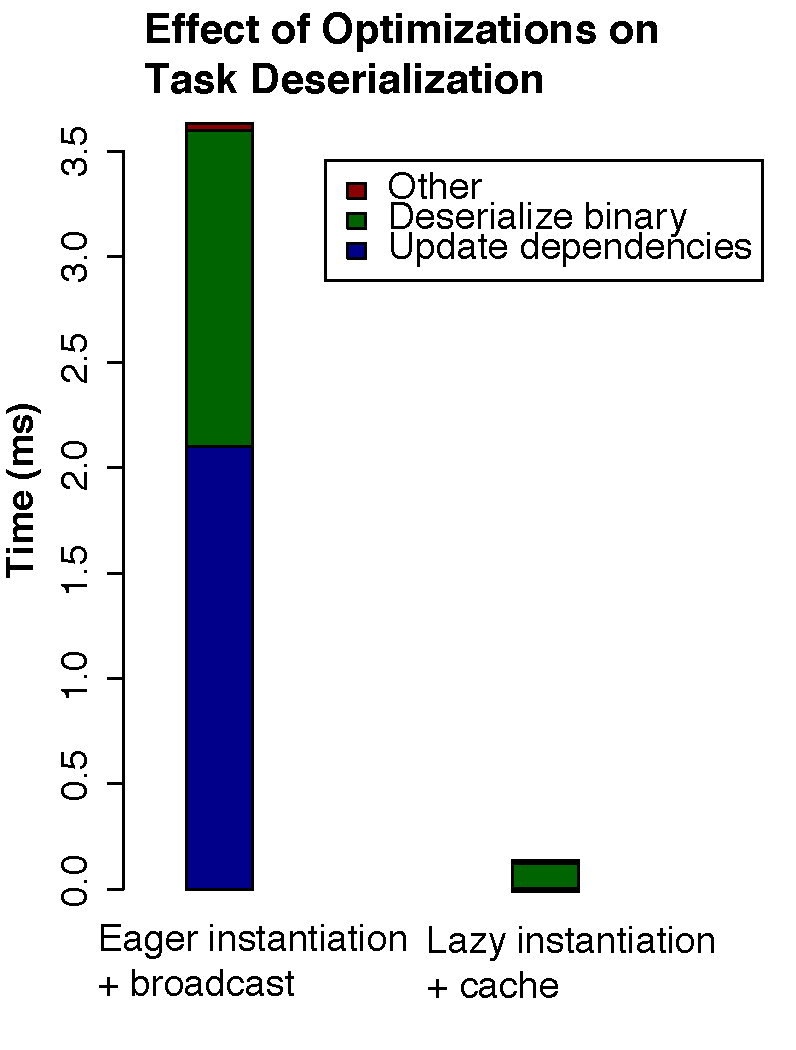
\includegraphics[scale=0.60]{images_graphs/optimizations/graph2/task_deser_micro.pdf}
 \end{center}
 \caption{Breakdown of averege time spent deserializing a task before and after adding lazy instantiation of configuration object and caching task binaries.}
 \label{fig:deserialization_times}
\end{figure}

Figure \ref{fig:deserialization_times} shows a time breakdown of deserialization. As can be seen in the graph, majority of the time in this case are in updating dependencies and deserializing \texttt{taskBytes}. We next examine each of these two components in more detail.

\subsubsection{Deserialize Binary}
In order to reduce the amount of duplicate data transferred, Spark 1.1.0 wraps the function and the RDD into a broadcast variable. This way, each executor will only fetch the function and the RDD of a batch once. The first task that uses the information will pull it from the driver, and cache the result within the executor for later tasks. In the Spark Streaming context however, this means for every stage, some task on every executor requires a round trip to the driver to fetch the broadcast variable, increasing the latency. As the batch interval shrinks, new RDDs are created more often, but the functions to operate on them do not change. The executor should be able to cache them for a longer period of time than only for the current stage.

To eliminate this round trip, we experimented with caching of \texttt{taskBytes}. The cache is implemented by keeping track of previously broadcasted \texttt{taskBytes} on the driver, and refer to their IDs instead of creating a new broadcast variable every time. Broadcast variables are automatically cached on the executor side, so this this methodology removes the extraneous communication with the driver.

\subsubsection{Update Dependencies}
In \texttt{updateDependencies()}, the current implementation creates a new Hadoop configuration object regardless of whether new dependencies are introduced. However, this objection creation is very costly in CPU cycles. Moreover, since a streaming application rarely introduces new dependencies once it starts to run, this method is incurring unnecessary costs. To solve this problem, we changed the object to be lazily instantiated, so that no cycles are spent creating the configuration object unless new dependencies are introduced.

\subsubsection{Evaluation}
The improvements of the two optimizations described above are also shown in Figure \ref{fig:deserialization_times}. After the changes, deserialization time for a task decreased from 3.6ms to 0.2ms. The impact of the two changes on overall task runtime is reflected in Figure \ref{fig:runtime_optimizations}.

\begin{figure}[t!]
 \begin{center}
   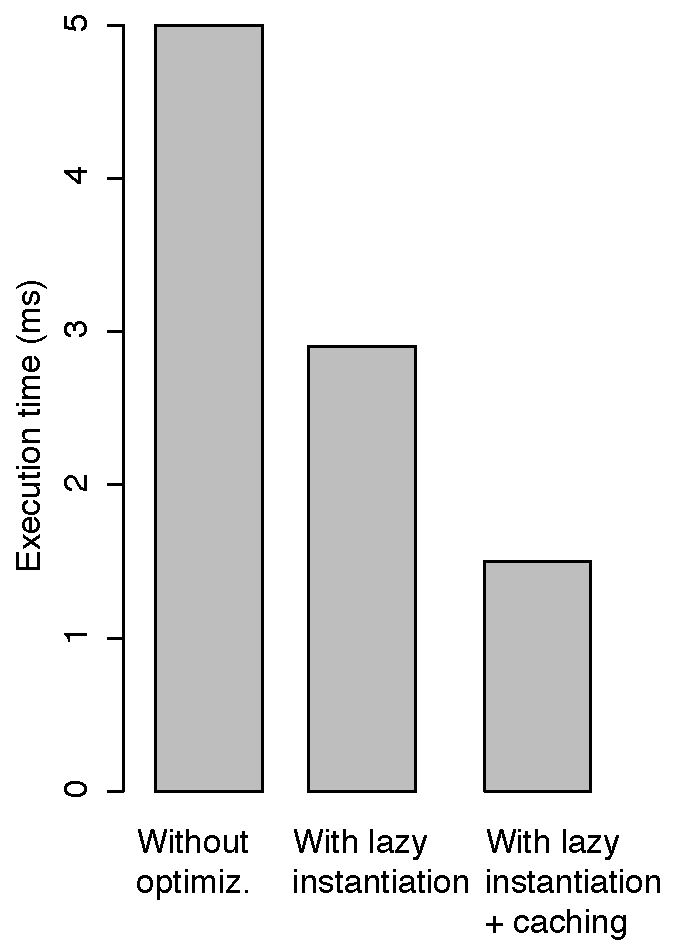
\includegraphics[scale=0.60]{images_graphs/optimizations/graph3/runtime_optimizations.pdf}
 \end{center}
 \caption{Average time spent in running no-op tasks before and after the optimizations in deserialization.}
 \label{fig:runtime_optimizations}
\end{figure}

To show the effect of reducing task runtimes, we performed a micro-benchmark running a single stage with many tasks. The results are shown in figure \ref{fig:lazy_macro}

\begin{figure}[t!]
 \begin{center}
   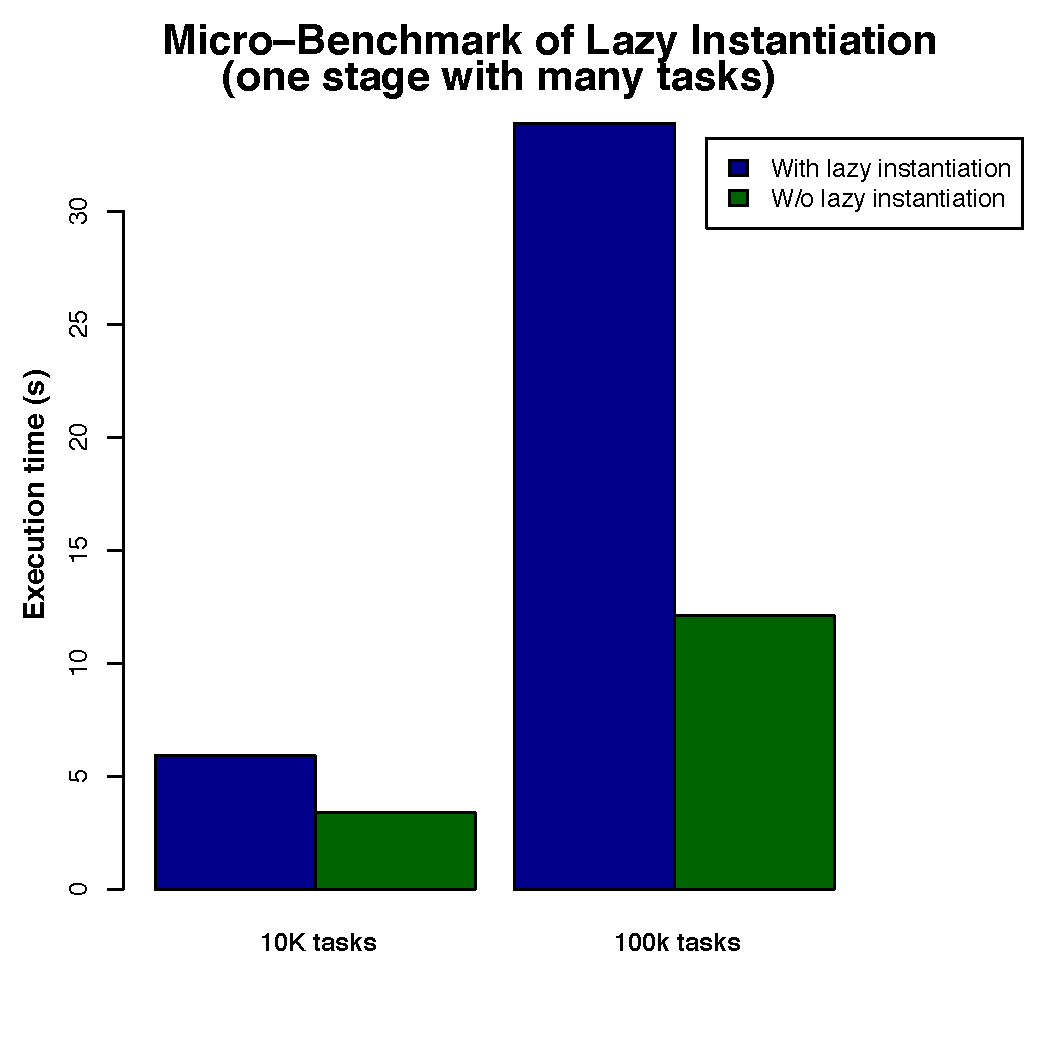
\includegraphics[scale=0.50]{images_graphs/optimizations/graph1/lazy_micro.pdf}
 \end{center}
 \caption{Amount of time spent running a single Spark stage consisting of many tasks without and with lazy instantiation of configuration object.}
 \label{fig:lazy_micro}
\end{figure}

\subsection{Limitations}
While caching task binaries sound simple in theory, they are more complicated to implement in practice. \team{Should we explain this in detail?}
